\documentclass[a4paper]{article}

% Set up page size
\usepackage[margin=1.5cm, includefoot, footskip=30pt]{geometry}

\usepackage{amsmath}
\usepackage{amsfonts}
\usepackage{hyperref}
\usepackage{minted}
\usepackage{graphicx}

\title{The evolution of the two thirds of the average game}
\author{Vince Knight and the students of MA3604}
\date{2022--03--24}

\begin{document}

\maketitle

\begin{abstract}
\end{abstract}

\section{Introduction}

The Two thirds of the game is a mathematical Parlour game that can be used to
introduce students to the concept of a Normal Form
Game~\cite{knight2015playing}.

In this game~\cite{maschler2020game}:

\begin{itemize}
    \item There are \(N\) players corresponding to every participant.
    \item The actions sets \(\mathcal{A}\) are the same for all players and
        correspond to guesses of natural numbers \(i \in \mathcal{A}\) between 0
        and 100 (inclusive).
    \item The utility is that the winners are the players who guessed closest to
        \(\frac{2}{3}\)rds of the average guess.
\end{itemize}

There are two Nash equilibrium (collections of strategies at which no player has
an incentive to deviate) for this game:

\begin{itemize}
    \item All players choosing \(0\): the two thirds of the average is \(0\) and
        thus all players win.
    \item All players choosing \(1\): the two thirds of the average is
        \(\frac{2}{3}\) and again all players win.
\end{itemize}

This game was originally described by a French magazine writer Alain Ledoux. As
the game corresponds not to choosing a number specific to the player but
reasoning about the guesses of the entire population it is also referred to as a
Keynesian beauty contests~\cite{mauersberger2020bounded}. This is due to a
similar situation where individuals were asked to rate photographs of people and
aim to identify the person who has the average preference.

The first author of this paper has used this game with students and at outreach
events collecting a large collection of guesses. A particularity of the approach
used~\cite{knight2015playing} is that the game is played twice, the second time
after having discussed and demonstrated the equilibria (although only the \(0\)
is discussed).

Figure~\ref{fig:history_of_play} shows the collected data. The second play of
the game does indicate a move towards one of the two equilibria.
In the next section of this paper, the replicator dynamics equation will be used
to explore whether or not this indication is an example of convergence towards
equilibria.

\begin{figure}[!hbtp]
    \centering
    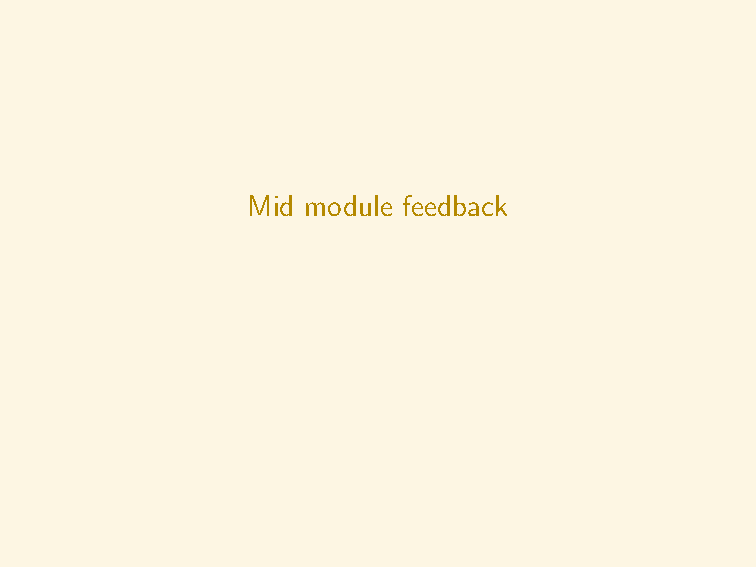
\includegraphics[width=.5\textwidth]{../static/main.pdf}
    \caption{A large collection of sequential plays of the game.}
    \label{fig:history_of_play}
\end{figure}

\section{Theory}

The replicator dynamics equation is a set of ordinary differential equations
that describe the evolution of a population of actions \(x\) in an evolutionary
setting. For a given vector \(x\in\mathbb{R}^n\) the replicator dynamics
equation is:

\begin{equation}\label{eqn:replicator-dynamics-equation}
    \frac{dx_i}{dt} = x_i(f_i - \phi)
\end{equation}

Where \(f_i\) is a measure of the fitness of individuals of type \(i\) and
\(\phi\) is the average of \(f_i\).

For the research described here the fitness function used is:

\begin{equation}
    f_i(x) = \frac{1}{1 + \left(i - \frac{2}{3}\sum_{i=0}^{N}ix_i\right) ^ 2}
\end{equation}

Note that this gives some fitness to individuals who do not win. The denominator
also includes a term to deal with discontinuity when the population is all
\(0\).

\section{Results}

The replicator dynamics equation~(\ref{eqn:replicator-dynamics-equation}) is
solved numerically using an algorithm described in~\cite{lind1983} and
implemented in the Fortran odepack interfaced via Scipy~\cite{scipy2020}.

The results are shown in Figure~\ref{fig:replicatory-dynamics} and it is clear
to see that the second equilibria emerges.

\begin{figure}[!hbtp]
    \centering
    \includegraphics[width=.7\textwidth]{../static/evolution.pdf}
    \caption{The outcome of the replicator dynamics equation.}
    \label{fig:replicatory-dynamics}
\end{figure}

\bibliographystyle{plain}
\bibliography{bibliography.bib}

\end{document}
